\begin{frame}{Доп.: Geometry Clipmaps}
    \begin{minipage}{.5\textwidth}
        \begin{itemize}
            \item Для ландшафта можно построить растровую карту высот
            \item Уменьшение детализации растровых изображений --- хорошо изученная задача
            \item По карте высот можно без разрывов рисовать геометрию разной детализации
        \end{itemize}
    \end{minipage}
    \begin{minipage}{.45\textwidth}
        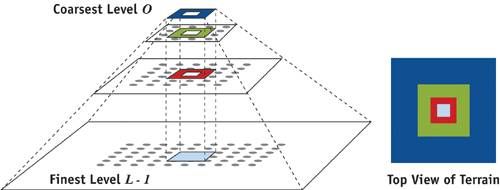
\includegraphics[width=\textwidth]{02_clipmaps_01.jpg}

        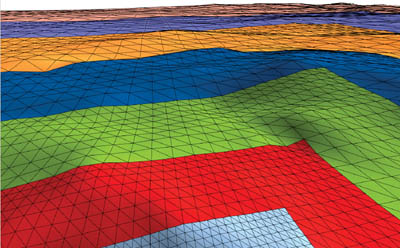
\includegraphics[width=\textwidth]{02_clipmaps_02.jpg}
    \end{minipage}
\end{frame}

\begin{frame}{Доп.: Sparse Voxel Octree}
    \centering
    \begin{minipage}{.75\textwidth}
        \begin{itemize}
            \item Меши приближают поверхность объекта
            \item Можно приближать не поверхность объекта, а его объём
            \item Воксель --- элементарная единица объёма
            \item Приближение объёма вокселями --- фактически, трёхмерное растровое изображение
            \item Одинаковые воксели группируются в кубы для экономии памяти и ускорения вычислений
        \end{itemize}
    \end{minipage}
    \begin{minipage}{.2\textwidth}
        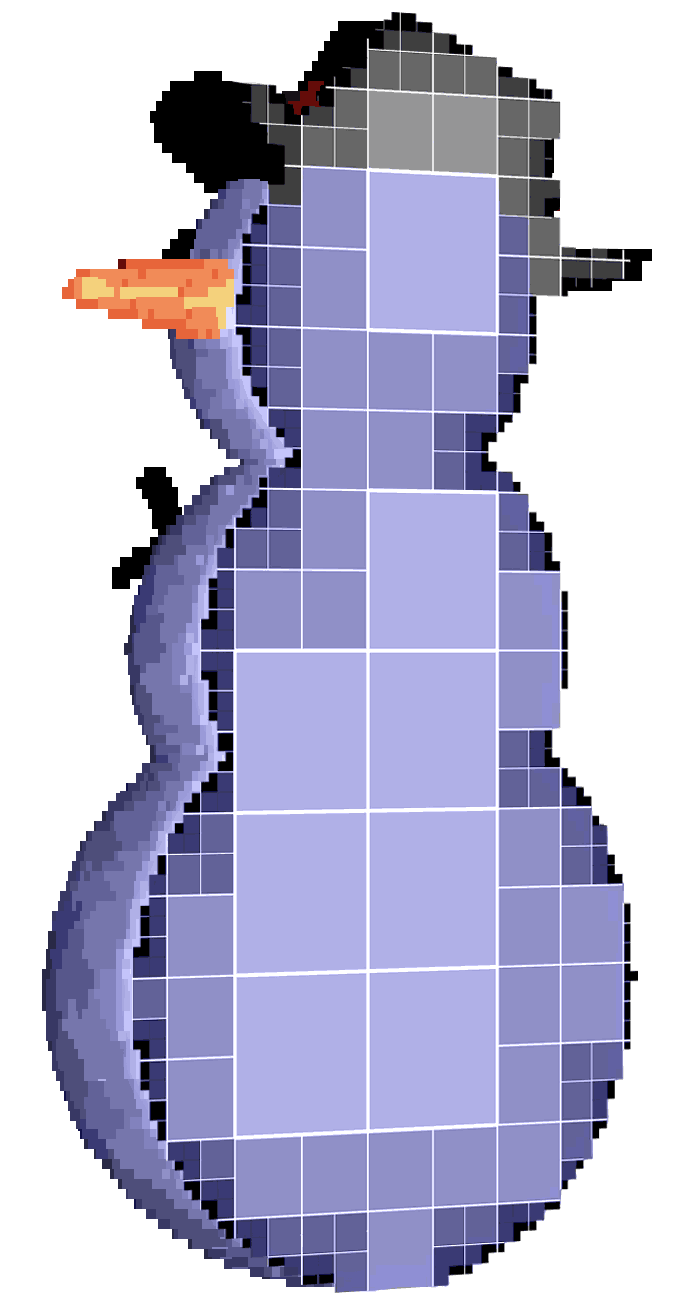
\includegraphics[width=\textwidth]{../Text/pics/SVO-voxel-snowman-slice-01.png}
    \end{minipage}
\end{frame}

\begin{frame}{Доп.: Плотность треугольников}
    \begin{center}
        \includegraphics[width=.45\textwidth]{../Text/pics/heatmap-mono.png}
        \includegraphics[width=.45\textwidth]{../Text/pics/heatmap-cluster.png}
        \includegraphics[width=.45\textwidth]{../Text/pics/heatmap-0.png}
    \end{center}
\end{frame}

\begin{frame}{Доп.: Исходный код}
    Исходный код доступен в GitHub-репозитории\\
    \url{https://github.com/asurkis/MasterThesis}

    \bigskip

    \begin{center}
        \qrcode[hyperlink,height=.5\textheight]{https://github.com/asurkis/MasterThesis}
    \end{center}
\end{frame}
